\documentclass{ximera}

 

\usepackage{epsfig}

\graphicspath{
  {./}
  {figures/}
}

\usepackage{morewrites}
\makeatletter
\newcommand\subfile[1]{%
\renewcommand{\input}[1]{}%
\begingroup\skip@preamble\otherinput{#1}\endgroup\par\vspace{\topsep}
\let\input\otherinput}
\makeatother

\newcommand{\includeexercises}{\directlua{dofile("/home/jim/linearAlgebra/laode/exercises.lua")}}

%\newcounter{ccounter}
%\setcounter{ccounter}{1}
%\newcommand{\Chapter}[1]{\setcounter{chapter}{\arabic{ccounter}}\chapter{#1}\addtocounter{ccounter}{1}}

%\newcommand{\section}[1]{\section{#1}\setcounter{thm}{0}\setcounter{equation}{0}}

%\renewcommand{\theequation}{\arabic{chapter}.\arabic{section}.\arabic{equation}}
%\renewcommand{\thefigure}{\arabic{chapter}.\arabic{figure}}
%\renewcommand{\thetable}{\arabic{chapter}.\arabic{table}}

%\newcommand{\Sec}[2]{\section{#1}\markright{\arabic{ccounter}.\arabic{section}.#2}\setcounter{equation}{0}\setcounter{thm}{0}\setcounter{figure}{0}}

\newcommand{\Sec}[2]{\section{#1}}

\setcounter{secnumdepth}{2}
%\setcounter{secnumdepth}{1} 

%\newcounter{THM}
%\renewcommand{\theTHM}{\arabic{chapter}.\arabic{section}}

\newcommand{\trademark}{{R\!\!\!\!\!\bigcirc}}
%\newtheorem{exercise}{}

\newcommand{\dfield}{{\sf dfield9}}
\newcommand{\pplane}{{\sf pplane9}}

\newcommand{\EXER}{\section*{Exercises}}%\vspace*{0.2in}\hrule\small\setcounter{exercise}{0}}
\newcommand{\CEXER}{}%\vspace{0.08in}\begin{center}Computer Exercises\end{center}}
\newcommand{\TEXER}{} %\vspace{0.08in}\begin{center}Hand Exercises\end{center}}
\newcommand{\AEXER}{} %\vspace{0.08in}\begin{center}Hand Exercises\end{center}}

% BADBAD: \newcommand{\Bbb}{\bf}

\newcommand{\R}{\mbox{$\Bbb{R}$}}
\newcommand{\C}{\mbox{$\Bbb{C}$}}
\newcommand{\Z}{\mbox{$\Bbb{Z}$}}
\newcommand{\N}{\mbox{$\Bbb{N}$}}
\newcommand{\D}{\mbox{{\bf D}}}
\usepackage{amssymb}
%\newcommand{\qed}{\hfill\mbox{\raggedright$\square$} \vspace{1ex}}
%\newcommand{\proof}{\noindent {\bf Proof:} \hspace{0.1in}}

\newcommand{\setmin}{\;\mbox{--}\;}
\newcommand{\Matlab}{{M\small{AT\-LAB}} }
\newcommand{\Matlabp}{{M\small{AT\-LAB}}}
\newcommand{\computer}{\Matlab Instructions}
\newcommand{\half}{\mbox{$\frac{1}{2}$}}
\newcommand{\compose}{\raisebox{.15ex}{\mbox{{\scriptsize$\circ$}}}}
\newcommand{\AND}{\quad\mbox{and}\quad}
\newcommand{\vect}[2]{\left(\begin{array}{c} #1_1 \\ \vdots \\
 #1_{#2}\end{array}\right)}
\newcommand{\mattwo}[4]{\left(\begin{array}{rr} #1 & #2\\ #3
&#4\end{array}\right)}
\newcommand{\mattwoc}[4]{\left(\begin{array}{cc} #1 & #2\\ #3
&#4\end{array}\right)}
\newcommand{\vectwo}[2]{\left(\begin{array}{r} #1 \\ #2\end{array}\right)}
\newcommand{\vectwoc}[2]{\left(\begin{array}{c} #1 \\ #2\end{array}\right)}

\newcommand{\ignore}[1]{}


\newcommand{\inv}{^{-1}}
\newcommand{\CC}{{\cal C}}
\newcommand{\CCone}{\CC^1}
\newcommand{\Span}{{\rm span}}
\newcommand{\rank}{{\rm rank}}
\newcommand{\trace}{{\rm tr}}
\newcommand{\RE}{{\rm Re}}
\newcommand{\IM}{{\rm Im}}
\newcommand{\nulls}{{\rm null\;space}}

\newcommand{\dps}{\displaystyle}
\newcommand{\arraystart}{\renewcommand{\arraystretch}{1.8}}
\newcommand{\arrayfinish}{\renewcommand{\arraystretch}{1.2}}
\newcommand{\Start}[1]{\vspace{0.08in}\noindent {\bf Section~\ref{#1}}}
\newcommand{\exer}[1]{\noindent {\bf \ref{#1}}}
\newcommand{\ans}{}
\newcommand{\matthree}[9]{\left(\begin{array}{rrr} #1 & #2 & #3 \\ #4 & #5 & #6
\\ #7 & #8 & #9\end{array}\right)}
\newcommand{\cvectwo}[2]{\left(\begin{array}{c} #1 \\ #2\end{array}\right)}
\newcommand{\cmatthree}[9]{\left(\begin{array}{ccc} #1 & #2 & #3 \\ #4 & #5 &
#6 \\ #7 & #8 & #9\end{array}\right)}
\newcommand{\vecthree}[3]{\left(\begin{array}{r} #1 \\ #2 \\
#3\end{array}\right)}
\newcommand{\cvecthree}[3]{\left(\begin{array}{c} #1 \\ #2 \\
#3\end{array}\right)}
\newcommand{\cmattwo}[4]{\left(\begin{array}{cc} #1 & #2\\ #3
&#4\end{array}\right)}

\newcommand{\Matrix}[1]{\ensuremath{\left(\begin{array}{rrrrrrrrrrrrrrrrrr} #1 \end{array}\right)}}

\newcommand{\Matrixc}[1]{\ensuremath{\left(\begin{array}{cccccccccccc} #1 \end{array}\right)}}



\renewcommand{\labelenumi}{\theenumi)}
\newenvironment{enumeratea}%
{\begingroup
 \renewcommand{\theenumi}{\alph{enumi}}
 \renewcommand{\labelenumi}{(\theenumi)}
 \begin{enumerate}}
 {\end{enumerate}\endgroup}



\newcounter{help}
\renewcommand{\thehelp}{\thesection.\arabic{equation}}

%\newenvironment{equation*}%
%{\renewcommand\endequation{\eqno (\theequation)* $$}%
%   \begin{equation}}%
%   {\end{equation}\renewcommand\endequation{\eqno \@eqnnum
%$$\global\@ignoretrue}}

%\input{psfig.tex}

\author{Martin Golubitsky and Michael Dellnitz}

%\newenvironment{matlabEquation}%
%{\renewcommand\endequation{\eqno (\theequation*) $$}%
%   \begin{equation}}%
%   {\end{equation}\renewcommand\endequation{\eqno \@eqnnum
% $$\global\@ignoretrue}}

\newcommand{\soln}{\textbf{Solution:} }
\newcommand{\exercap}[1]{\centerline{Figure~\ref{#1}}}
\newcommand{\exercaptwo}[1]{\centerline{Figure~\ref{#1}a\hspace{2.1in}
Figure~\ref{#1}b}}
\newcommand{\exercapthree}[1]{\centerline{Figure~\ref{#1}a\hspace{1.2in}
Figure~\ref{#1}b\hspace{1.2in}Figure~\ref{#1}c}}
\newcommand{\para}{\hspace{0.4in}}

\renewenvironment{solution}{\suppress}{\endsuppress}

\ifxake
\newenvironment{matlabEquation}{\begin{equation}}{\end{equation}}
\else
\newenvironment{matlabEquation}%
{\let\oldtheequation\theequation\renewcommand{\theequation}{\oldtheequation*}\begin{equation}}%
  {\end{equation}\let\theequation\oldtheequation}
\fi

\makeatother


\title{Examples of Bifurcations}

\begin{document}
\begin{abstract}
\end{abstract}
\maketitle


\label{S:bifurcation} \index{bifurcation}

In Section~\ref{S:TSPM} we illustrated how modeling leads to systems 
of differential equations that depend on external parameters.  In this 
section we discuss some of the expected ways in which phase portraits of 
systems of differential equations change as a single parameter is varied.  
These ways include changes in the number of equilibria and in the number 
of limit cycles, and are called {\em bifurcations\/}.   We use simple 
differential equations to illustrate three different kinds of bifurcation: 
{\em saddle-node\/} bifurcations where two equilibria collide and disappear; 
{\em Hopf\/} bifurcations where limit cycles are created; and 
{\em homoclinic\/} bifurcations where limit cycles disappear.  We also show 
how to use {\em bifurcation diagrams\/} to summarize these changes.

\subsection*{Saddle-Node Bifurcations on the Line}
\index{bifurcation!saddle-node}

Consider the differential equation
\begin{equation}  \label{E:sbif}
\dot{x} = \rho - x^2 \equiv f(x,\rho).
\end{equation}
We discuss how the phase line to \eqref{E:sbif} changes as $\rho$ increases 
through $0$.  A simple numerical experiment using {\sf pline} shows that
the phase lines for \eqref{E:sbif} when $\rho=-1,0,1$ are those given in 
Figure~\ref{F:sbif}.  From this figure we see that a pair of equilibria 
is created as $\rho$ increases through $0$.

\vspace{0.4in}

\begin{figure*}[htb]
           \centerline{%
           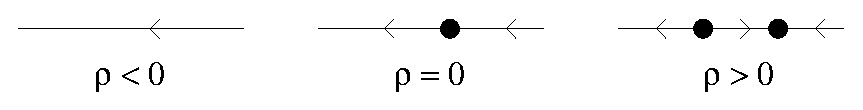
\psfig{file=../figures/sbif.eps,width=6.0in}}
           \caption{Phase lines for the differential equation 
    		\protect\eqref{E:sbif}.}
           \label{F:sbif}
\end{figure*}\index{phase!line}


These phase lines can be verified analytically by solving the 
algebraic equation $f(x,\rho)=0$ and obtaining:
\begin{equation} \label{E:sbife}
x^2 = \rho.
\end{equation}
When $\rho<0$ there are no (real) solutions to \eqref{E:sbife}; when
$\rho=0$ the only solution to \eqref{E:sbife} is $x=0$; and when $\rho>0$
there are two solutions to \eqref{E:sbife} given by $x=\pm\sqrt{\rho}$.
It follows that \eqref{E:sbif} has no equilibria when $\rho<0$, a single
equilibrium when $\rho=0$, and two equilibria when $\rho>0$.

Additionally, we can determine the stability\index{stability}
of the equilibria using 
Theorem~\ref{T:stability1} in Chapter~\ref{chap:SolveOdes}.  Observe that
\[
f_x(x,\rho) = -2x.
\]
Therefore, $f_x<0$ at $x=\sqrt{\rho}$ and $f_x>0$ at $x=-\sqrt{\rho}$.
Theorem~\ref{T:stability1} implies that the equilibrium at $x=-\sqrt{\rho}$ 
is unstable and that the equilibrium at $x=\sqrt{\rho}$ is stable.

We summarize the information about equilibria of \eqref{E:sbif} in the 
bifurcation diagram\index{diagram!bifurcation} in Figure~\ref{F:sbifBIF}.  
This bifurcation diagram is formed as follows: graph the points where 
$f(x,\rho)=0$ in the $\rho x$ plane; that is, graph the parabola $\rho=x^2$.  
On that graph we use a solid line when the equilibrium of \eqref{E:sbif} is 
stable and a dashed line when the equilibrium is unstable.

\begin{figure}[htb]
           \centerline{%
           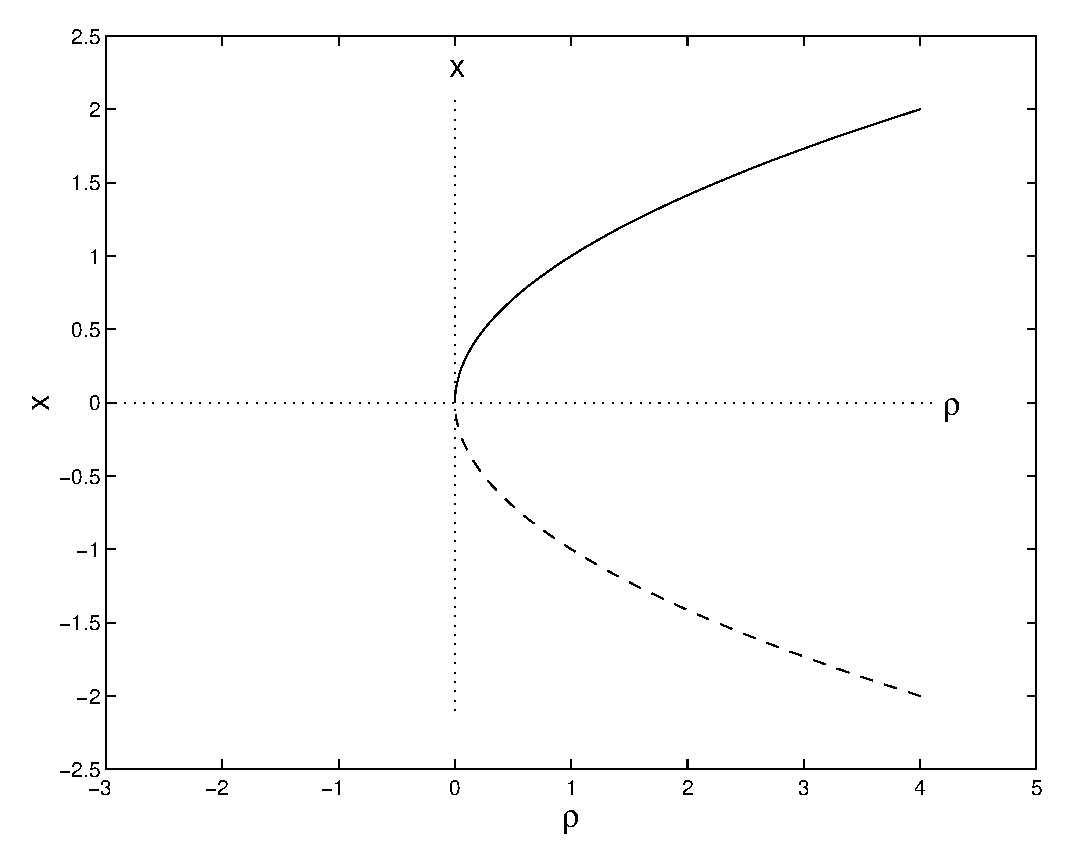
\psfig{file=../figures/sbifBIF.eps,width=4.0in}}
           \caption{Bifurcation diagram for the differential equation
        \protect\eqref{E:sbif}. }
           \label{F:sbifBIF}
\end{figure}

We have shown that at $\rho=0$ the differential equation \eqref{E:sbif} 
undergoes a saddle-node bifurcation\index{bifurcation!saddle-node}
where a pair of equilibria is created.  Moreover, one of this pair is stable 
and one is unstable.  Next, we consider a more complicated example:
\begin{equation} \label{E:cbif}
\dot{x} = \rho - x^3 + 3x \equiv f(x,\rho).
\end{equation}
We can solve for the equilibria of this differential equation by solving
the algebraic equation $f(x,\rho)=0$ for
\begin{equation}  \label{E:rho=cubic}
\rho = x^3 - 3x.
\end{equation}
Graphing \eqref{E:rho=cubic} in the $\rho x$ plane yields the bifurcation 
diagram in Figure~\ref{F:cbifBIF}.  Note that two equilibria appear at 
$\rho=-2$ as $\rho$ increases and that two equilibria disappear at 
$\rho=2$.  Thus, there are two saddle-node bifurcations for \eqref{E:cbif}: 
one at $\rho=-2$ and one at $\rho=2$.

\begin{figure}[htb]
           \centerline{%
           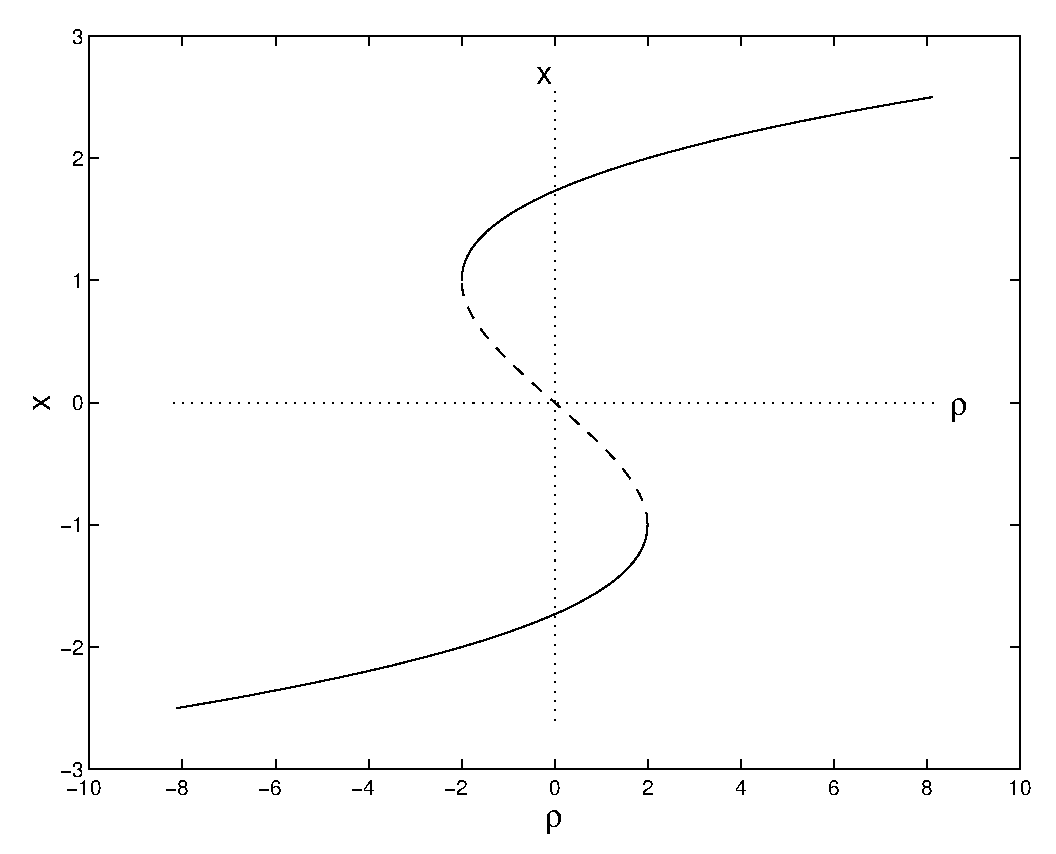
\psfig{file=../figures/cbifBIF.eps,width=4.0in}}
           \caption{Bifurcation diagram for the differential equation
        \protect\eqref{E:cbif}.}
           \label{F:cbifBIF}
\end{figure} \index{diagram!bifurcation}

In Figure~\ref{F:cbifBIF} we have again plotted stable equilibria
\index{equilibrium!stable} using solid lines and unstable equilibria
\index{equilibrium!unstable} using dashed lines.  The
stability can be checked analytically by computing
\[
f_x(x,\rho) = -3x^2+3 = 3(1-x^2).
\]
It follows that $f_x<0$ at equilibria where $|x|>1$ and $f_x>0$ at 
equilibria where $|x|<1$.  So the equilibria at $x$ values between 
$-1$ and $1$ are unstable and the equilibria at $x>1$ and $x<-1$ are 
stable.  The phase lines are those given in Figure~\ref{F:cbif}.  These 
calculations can be verified using {\sf pline}. 

\vspace{0.4in}

\begin{figure*}[htb]
           \centerline{%
           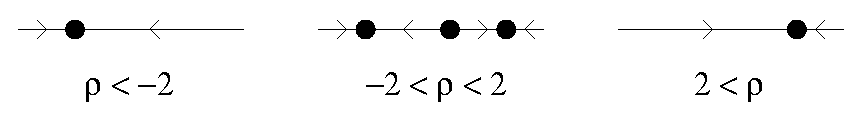
\psfig{file=../figures/cbif.eps,width=6.0in}}
           \caption{Phase lines for the differential equation
        \protect\eqref{E:cbif}.}
           \label{F:cbif}
\end{figure*}

\subsubsection*{The Detection of 1-D Saddle-Node Bifurcations}

In differential equations of the form
\[
\dot{x} = f(x,\rho)
\]
we have seen that at points $(x_0,\rho_0)$ where saddle-node bifurcations
occur two equilibria collide as the parameter $\rho$ is varied, and one of 
these equilibria is stable while the other one is unstable.  Therefore, the
following restrictions on $f$ must hold:
\begin{equation}  \label{E:DCSN}
\begin{array}{rcl}
f(x_0,\rho_0) & = & 0\\
f_x(x_0,\rho_0) & = & 0.
\end{array}
\end{equation}
The first condition just states that the point $(x_0,\rho_0)$ is an
equilibrium of the differential equation.  The second condition follows from
continuity; there are two equilibria nearby one of which is asymptotically 
stable $f_x<0$ and the other is unstable $f_x>0$.  In between, which means at
the point $(x_0,\rho_0)$, we must have $f_x=0$.

For example, we can find points where saddle-node bifurcations might occur in 
the differential equation:
\[
\dot{x} = 2x^2 +\rho x + 2
\]
by solving the two equations given in \eqref{E:DCSN}.  Set 
\[
f(x,\rho) = 2x^2 +\rho x + 2
\]
and differentiate to obtain
\[
f_x(x,\rho) = 4x + \rho.
\]
On setting $f_x=0$ we find
\[
\rho = -4x.
\]
Substituting this result into the equation $f=0$ yields
\[
-2x^2 + 2 =0
\]
which can be solved for $x=\pm 1$.  There are two possible points where
saddle-node bifurcations can occur; they are:
\[
(x_0,\rho_0) = (1,-4) \AND  (x_0,\rho_0) = (-1,4).
\]
It can be checked using {\sf pline} that saddle-node bifurcations do actually
occur at both points.

Conditions \eqref{E:DCSN} are necessary conditions for the existence of a 
saddle-node bifurcation; by themselves they are not sufficient.  For example, 
consider
\[
f(x,\rho) = x^2 -\rho^2.
\]
Since $f(0,0)=0$ and $f_x(0,0)=0$, the origin satisfies \eqref{E:DCSN}.  But 
the bifurcation is not a saddle-node bifurcation as there 
are two equilibria for every nonzero value of $\rho$.

\subsection*{Saddle-Node Bifurcations in the Plane}
\index{bifurcation!saddle-node!in the plane}

The transition from no equilibria to two equilibria can occur as a 
parameter is varied in differential equations with any number of 
variables.  Here we consider one example of a planar system of 
differential equations where a saddle-node bifurcation occurs.
Consider the system of differential equations 
\begin{matlabEquation}  \label{E:ssys}
\begin{array}{rcl}
\dot{x} & = & x^2 - \rho + y \\
\dot{y} & = & -y(x^2+1).  \end{array}
\end{matlabEquation}

From the $\dot{y}$ equation we see that equilibria only occur 
when $y=0$.  Substituting $y=0$ into the $\dot{x}$ equation yields
the equation $x^2=\rho$.   Thus there are no equilibria for $\rho<0$;
a single equilibrium at the origin for $\rho=0$; and two equilibria
at 
\[
X_{\pm}=(\pm\sqrt{\rho},0)
\]
for $\rho>0$.  The bifurcation diagram 
for the system of differential equations \eqref{E:ssys} is identical to
the one for the single equation \eqref{E:sbif} given in Figure~\ref{F:sbif}.

In Figure~\ref{F:ssys}, the phase portraits of \eqref{E:ssys} are given for 
two values of $\rho$; namely, $\rho=-1$ and $\rho=1$.  Note that when 
$\rho=0$ the origin is a nonhyperbolic 
equilibrium\index{equilibrium!nonhyperbolic} and when $\rho=1$
the equilibrium at $(-1,0)$ is a nodal sink\index{nodal sink} 
while the equilibrium at 
$(1,0)$ is a saddle\index{saddle}.  
Thus this saddle-node bifurcation creates a saddle 
and a nodal sink.  In all planar saddle-node bifurcations one of the 
equilibria will be a saddle and the other will either be a nodal source 
or a nodal sink.  See Exercise~\ref{e:source}.

\begin{figure*}[htb]
           \centerline{%
           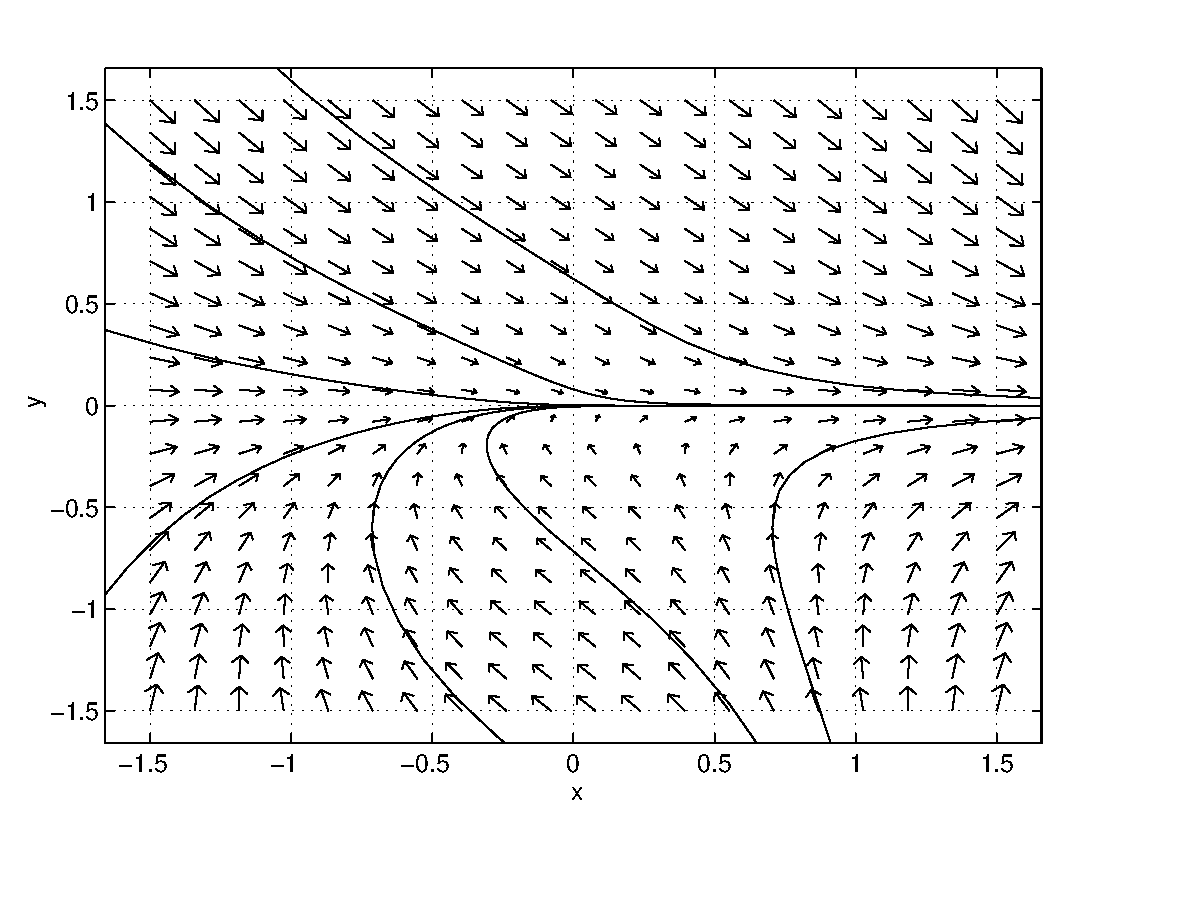
\psfig{file=../figures/ssys1.eps,height=2.0in}
	   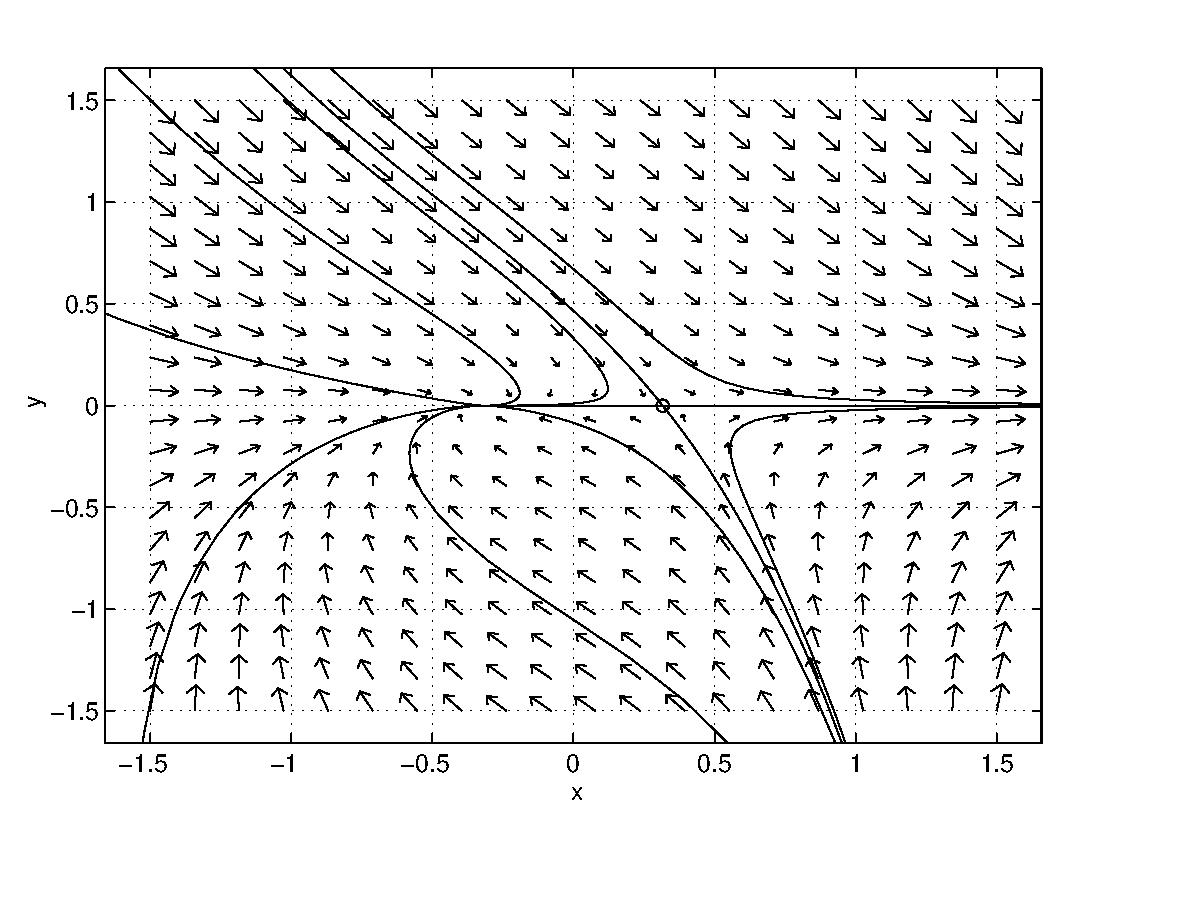
\psfig{file=../figures/ssys3.eps,height=2.0in}}
		\vspace*{-0.2in}		
		\hspace{1.3in} $\rho=-1$ \hspace{2.1in} $\rho=1$
   \caption{Phase planes for the differential equation \protect\eqref{E:ssys}.}
           \label{F:ssys}
\end{figure*}

It is instructive to determine the type of equilibria in \eqref{E:ssys} by
computing the Jacobian matrix.  Let $F(x,y)$ denote the right hand side of 
\eqref{E:ssys} and calculate:
\begin{equation}  \label{E:SNJ}
dF = \mattwoc{2x}{1}{-2xy}{-x^2-1} \AND 
(dF)_{X_{\pm}}= \mattwoc{\pm 2\sqrt{\rho}}{1}{0}{-\rho-1}.
\end{equation}
Observe that when $\rho=0$ the linearized differential equation, at the origin, 
is the nonhyperbolic saddle-node
\[
\dot{X} = \mattwo{0}{1}{0}{-1}X,
\]
whose eigenvalues are $0$ and $1$.  See Section~\ref{S:6.9}. We can also check
using \eqref{E:SNJ} that when $\rho>0$ the linearization at $X_{-}$ has two 
negative real eigenvalues ($-2\sqrt{\rho}$ and $-\rho-1$)  and is a node 
while the linearization at $X_{+}$ has one positive ($2\sqrt{\rho}$) and one 
negative ($-\rho-1$) eigenvalue and is a saddle.


\subsubsection*{Detection of 2D Saddle-Node Bifurcations}

Saddle-node bifurcations occur in planar systems at equilibria  where a 
saddle and a node coalesce.  Consider the planar system of differential 
equations
\[
\dot{X} = F(X,\rho).
\]
At a saddle-node bifurcation point $(X_0,\rho_0)$, the following conditions
must be satisfied:
\begin{equation}  \label{E:DCSN2}
\begin{array}{rcl}
F(X_0,\rho_0) & = & 0\\
\det(J) & = & 0.
\end{array}
\end{equation}
where $J = (dF)_{(X_0,\rho_0)}$ satisfies $\trace(J)\neq 0$.  The first 
equation just states that $(X_0,\rho_0)$ is an equilibrium and the second 
equation implies that the Jacobian has a zero eigenvalue.  Since 
$\trace(J)\neq 0$, $J$ has a nonzero eigenvalue and is a saddle-node matrix.

We can use \eqref{E:DCSN2} to find possible saddle-node bifurcation points in
planar systems.  For example, consider the system
\[
\begin{array}{rcl} 
\dot{x} & = & x^2 + y^2 - \rho\\
\dot{y} & = & x + y -2.
\end{array}
\]
The two parts of \eqref{E:DCSN2} lead to three equations:
\[
\begin{array}{rcl} 
x^2 + y^2 - \rho & = & 0\\
x + y -2 & = 0\\
\det\mattwoc{2x}{2y}{1}{1} & = & 0.
\end{array}
\]
These equations can be solved for $(x_0,y_0,\rho_0)=(1,1,2)$.  Indeed, for 
$\rho\approx 2$, {\pplane} can be used to show that there are two 
equilibria near $(1,1)$ (a saddle and a node) when $\rho>2$ and no 
equilibria near $(1,1)$ when $\rho<2$.



\subsection*{Hopf Bifurcation in a Planar System} 
\index{bifurcation!Hopf}

Another type of bifurcation that can occur in planar systems (though not in
single autonomous equations) is the creation of a limit cycle from an
equilibrium.  This type of bifurcation is commonly called {\em Hopf 
bifurcation\/}.  We begin our discussion with a numerical example.  

Load the planar system of differential equations 
\begin{matlabEquation} \label{E:Hopfbif}
\begin{array}{rcl}
\dot{x} & = & y \\
\dot{y} & = & -x + \rho y - y^3  \end{array}
\end{matlabEquation}
into {\pplane}.
It is straightforward to see that the origin is an equilibrium of 
\eqref{E:Hopfbif} for all values of $\rho$ --- indeed, the origin is 
the only equilibrium of \eqref{E:Hopfbif}.  Now plot the phase 
portraits for $\rho=-1$ and $\rho=1$.  These plots are shown in 
Figure~\ref{F:Hopfbif}.  

\begin{figure*}[htb]
           \centerline{%
           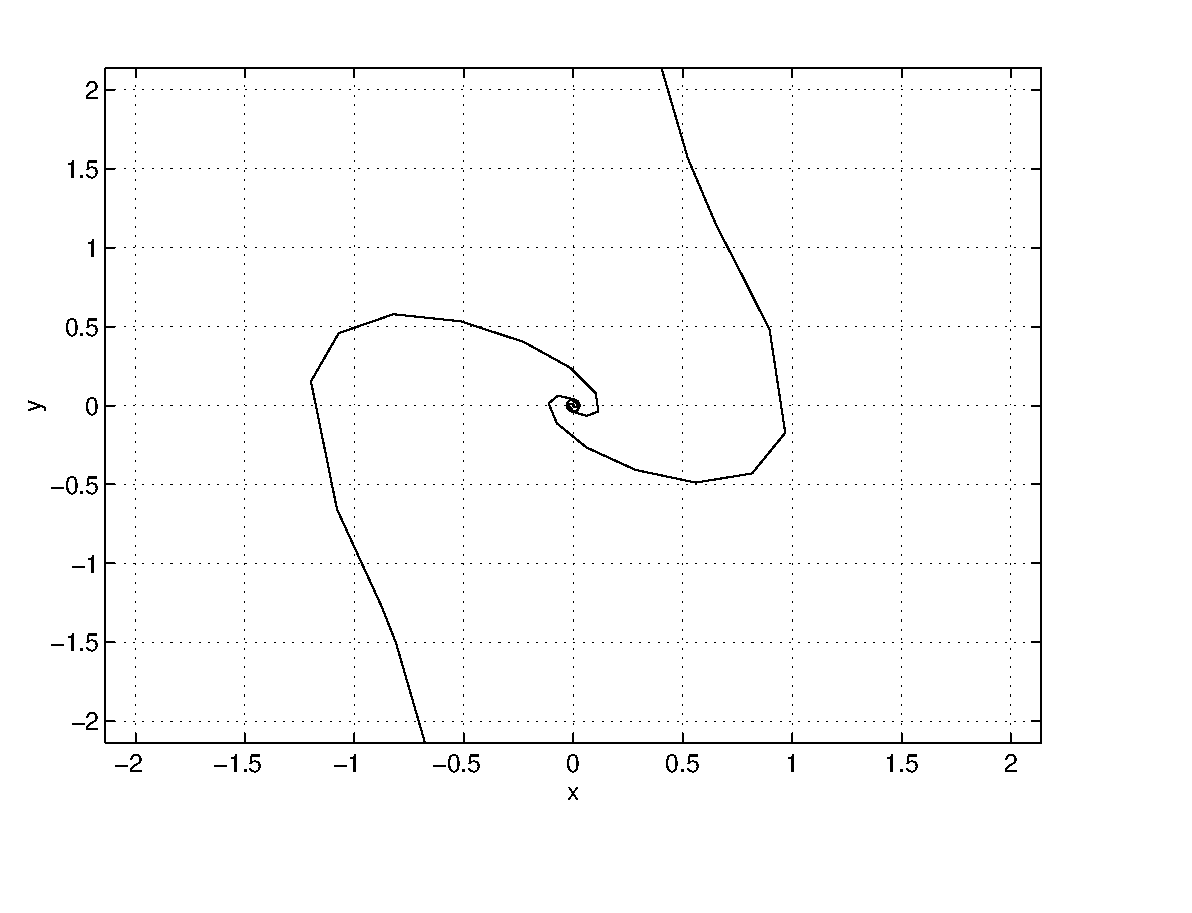
\psfig{file=../figures/Hopfbif1.eps,height=2.5in}
           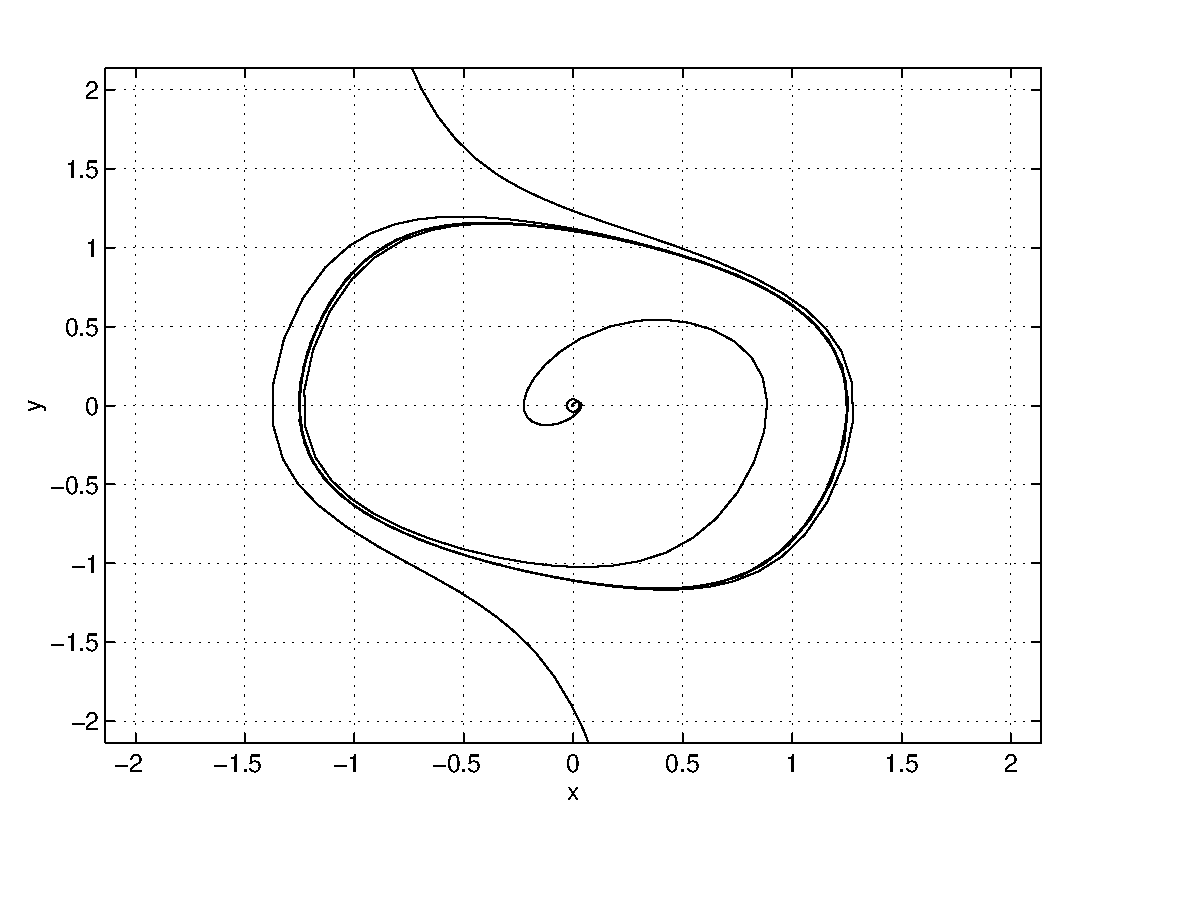
\psfig{file=../figures/Hopfbif2.eps,height=2.5in}}
		\vspace*{-0.2in}		
		\qquad\qquad\qquad $\rho=-1$ \hspace{2.8in} $\rho=1$
	   \caption{Phase planes for the differential equation 
      \protect\eqref{E:Hopfbif}.}
           \label{F:Hopfbif}
\end{figure*}


The Jacobian of \eqref{E:Hopfbif} at the origin is:
\[
\mattwoc{0}{1}{-1}{\rho}.
\]
It follows that the origin goes from being a 
spiral sink\index{sink} to being a 
spiral source\index{source} 
as $\rho$ increases through $0$.  It also follows that  
the origin is a center\index{center} at $\rho=0$.  
The main new feature of the phase portraits is the 
existence of an asymptotically stable\index{stability!asymptotic} 
periodic solution when $\rho>0$.  
Hopf bifurcations can also produce unstable periodic solutions
\index{periodic solution!unstable} (see \eqref{E:hopfdetect} for an example).   

\subsubsection*{Bifurcation Diagrams for Hopf Bifurcation}

There are two salient points concerning Hopf bifurcation.  The first point is 
that a spiral sink equilibrium loses stability and becomes a spiral source 
as a parameter is varied (or vice versa).  The second point is that a limit
cycle (either stable or unstable) is produced by this change in stability. 
We draw schematic bifurcation diagrams in
Figures~\ref{F:Hopfbifdiag}--\ref{F:Hopfbifdiag2} to indicate this change.  
On this diagram stable equilibria are indicated by a 
solid line and unstable equilibria are indicated by a dashed line, as before.
Stable limit cycles are indicated by a heavy dotted line and unstable limit 
cycles are indicated by a dot-dashed line.  Note that the bifurcation diagram
in Figure~\ref{F:Hopfbifdiag} describes the Hopf bifurcation in the system of
differential equations \eqref{E:Hopfbif}. 

\begin{figure}[htb]
           \centerline{%
           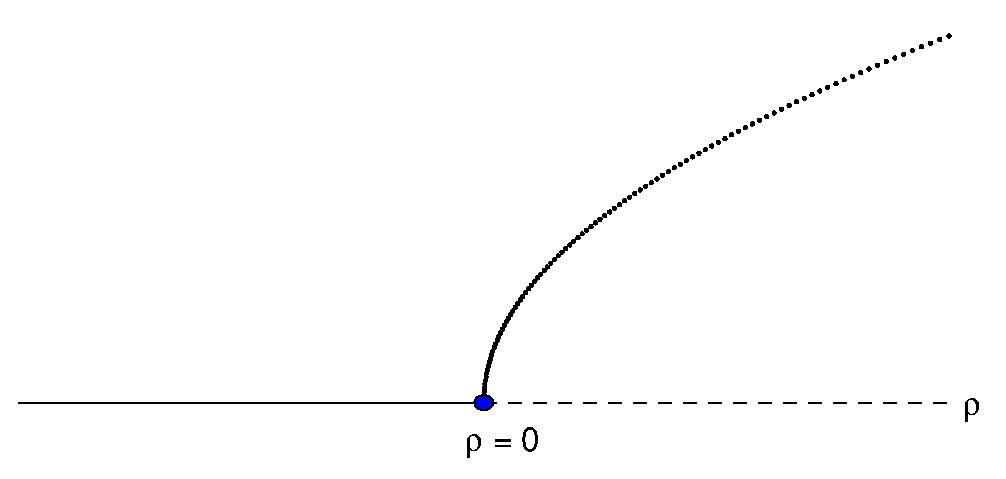
\psfig{file=../figures/Hopfbifa.eps,height=1.6in}}
  \caption{Schematic bifurcation diagram for the differential equation 
    \protect\eqref{E:Hopfbif} with a branch of stable limit cycles emanating 
	from a point of Hopf bifurcation indicated by a dotted line.}
           \label{F:Hopfbifdiag}
\end{figure}
\index{diagram!bifurcation}

\begin{figure}[htb]
           \centerline{%
           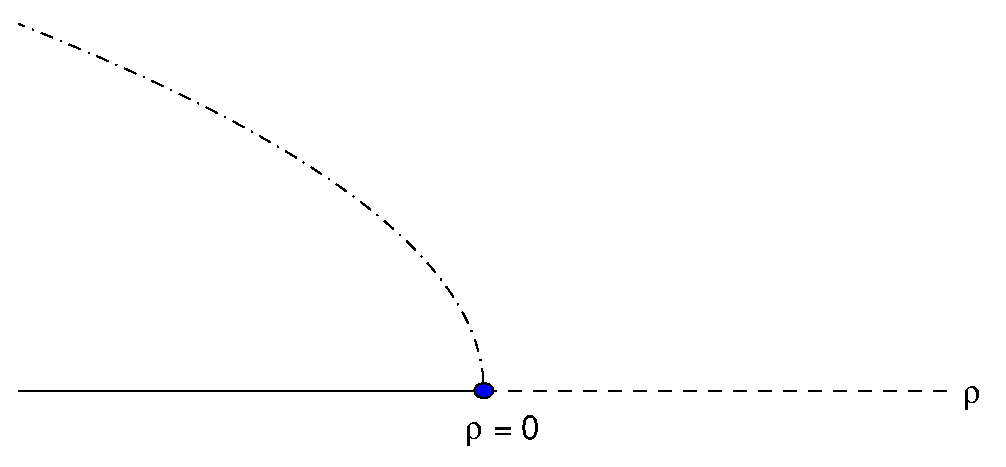
\psfig{file=../figures/Hopfbifb.eps,height=1.6in}}
  \caption{Schematic bifurcation diagram with a branch of unstable limit 
	cycles emanating from a point of Hopf bifurcation indicated by a 
	dot-dashed line.}
           \label{F:Hopfbifdiag2}
\end{figure}
\index{diagram!bifurcation}

\subsubsection*{Detection of Hopf Bifurcations}

A necessary condition for producing a limit cycle from an equilibrium by
varying an external parameter is the existence of an equilibrium whose
linearization is a center.  Thus, $(X_0,\rho_0)$ is a possible point of 
Hopf bifurcation for the planar system
\[
\dot{X} = F(X,\rho)
\]
if the following conditions are satisfied:
\begin{equation} \label{E:NCHB}
\begin{array}{rcl}
F(X_0,\rho_0) & = & 0\\
\trace(J) & = & 0\\
\det(J) & > & 0
\end{array}
\end{equation}
where $J= (dF)_{(X_0,\rho_0)}$.

We can use \eqref{E:NCHB} to find possible points of Hopf bifurcation.  For 
example, consider the system
\begin{matlabEquation}  \label{E:hopfdetect}
\begin{array}{rcl}
\dot{x} & = & 2y - \rho + x^2 - 2y^2\\
\dot{y} & = & -x + y^2.
\end{array}
\end{matlabEquation}
A point of Hopf bifurcation in \eqref{E:hopfdetect} must satisfy the three 
equations
\[
\begin{array}{rcl}
2y - \rho  + x^2 - 2y^2 & = & 0\\
-x + y^2 & = & 0 \\
2(x + y)  & = & 0,
\end{array}
\]
where, in addition, $\det(J) = 4xy+2-4y>0$.  It follows from the third 
equation ($\trace(J)=0$) that $y=-x$.  On substitution for $y$ in the first 
two equations, we find
\[
\begin{array}{rcl}
-2x - \rho - x^2 & = & 0\\
-x + x^2 & = & 0,
\end{array}
\]
where $\det(J) = -4x^2+4x+2$.  From the second equation it follows that $x=0$
or $x=1$.  So there are two solutions to this system of equations: 
$(x_0,y_0,\rho_0)=(0,0,0)$ and $(x_1,y_1,\rho_1)=(1,-1,-3)$.  At both of
these points the determinant of the Jacobian matrix is $2$.  Hence the
linearized equations at both point are centers, and there are two possible
points of Hopf bifurcation.

Numerical exploration of \eqref{E:hopfdetect} using {\pplane} shows that 
there are unstable limit cycles emanating from both of these points; hence 
there are exactly two points of Hopf bifurcation in this system of equations.



\subsection*{Conventions for Bifurcation Diagrams}

In all bifurcation diagrams we will indicate
\begin{itemize}
\item	stable equilibria by a solid line;
\item	unstable equilibria by a dashed line;
\item	stable limit cycles by a dotted line;
\item	unstable limit cycles by a dot-dashed line; and
\item	bifurcation points by black circles.
\end{itemize}

For example, the information contained in the Hopf bifurcation of 
\eqref{E:Hopfbif} is summarized by the bifurcation diagram in 
Figure~\ref{F:Hopfbifdiag}.
In that figure, a curve of equilibria \index{curve of equilibria} 
loses stability at $\rho=0$ as $\rho$ increases.  A branch of limit 
cycles\index{limit cycle!branch of} emanates from the
branch of equilibria at the bifurcation point, which is indicated by a 
black dot.  The stable limit cycles are indicated by the dotted line.



\subsection*{Homoclinic Bifurcations}
\index{bifurcation!homoclinic}

There is a second way that planar systems of differential equations 
can have periodic solutions appear or disappear as parameters are varied.  
This  change is called a {\em homoclinic bifurcation\/}.  For example,
consider the system of differential equations
\begin{matlabEquation}  \label{E:homobif}
\begin{array}{rcl} 
\dot{x} & = & \rho x - y \\
\dot{y} & = &  x + x^2 + xy.
\end{array}
\end{matlabEquation}
Begin by noting that the origin is an equilibrium of \eqref{E:homobif}
for every value of $\rho$ and the linearized equation about this equilibrium 
is:
\[
\dot{X} = \mattwo{\rho}{-1}{1}{0}X.
\]
It follows that \eqref{E:homobif} has a Hopf bifurcation at the origin, as 
the origin changes from a spiral sink to a spiral source as $\rho$ 
increases through zero.  Calculations show that \eqref{E:homobif} has a 
second equilibrium at 
\[
X_0 = -\frac{1}{1+\rho}(1,\rho)
\]
and that this equilibrium is a saddle when $\rho>-1$.

\begin{figure*}[htb]
           \centerline{%
           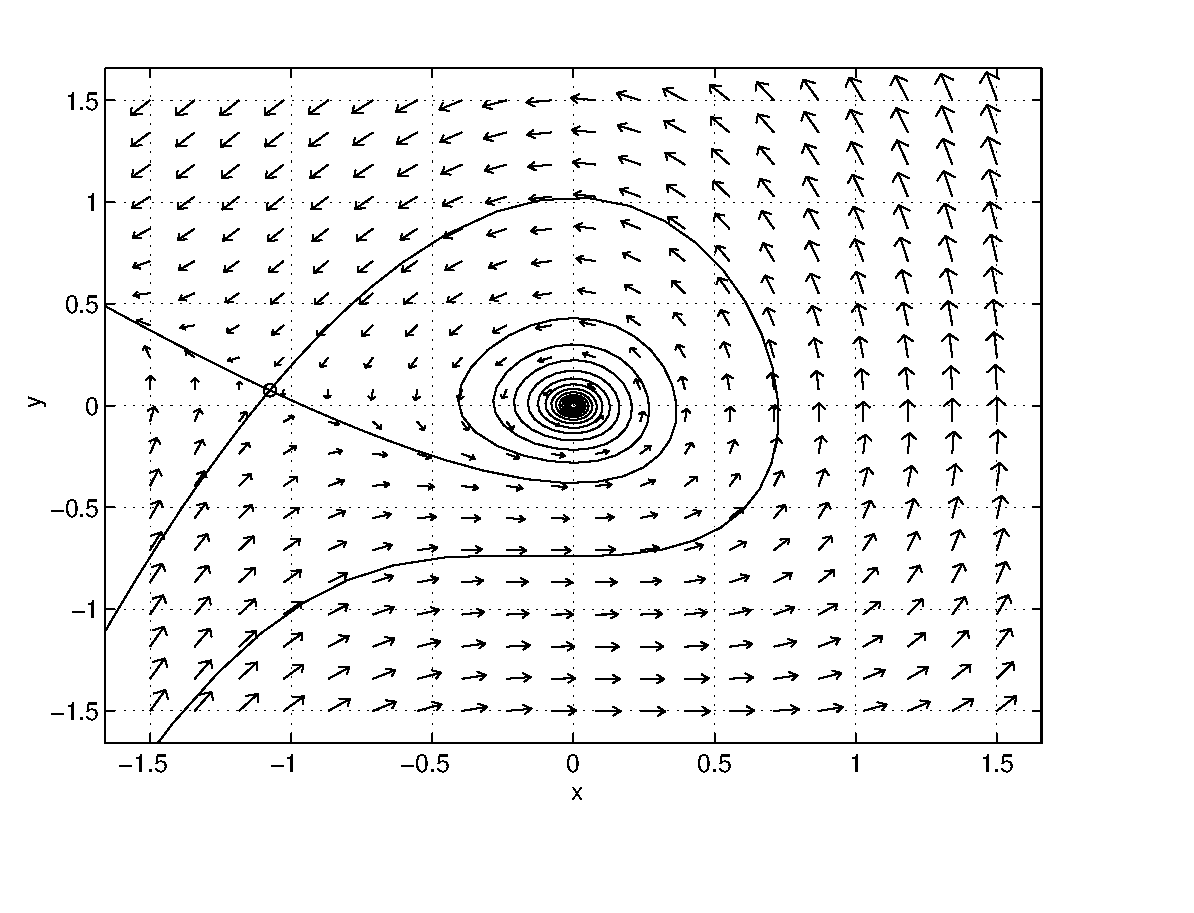
\psfig{file=../figures/homobif1.eps,height=2.0in}
           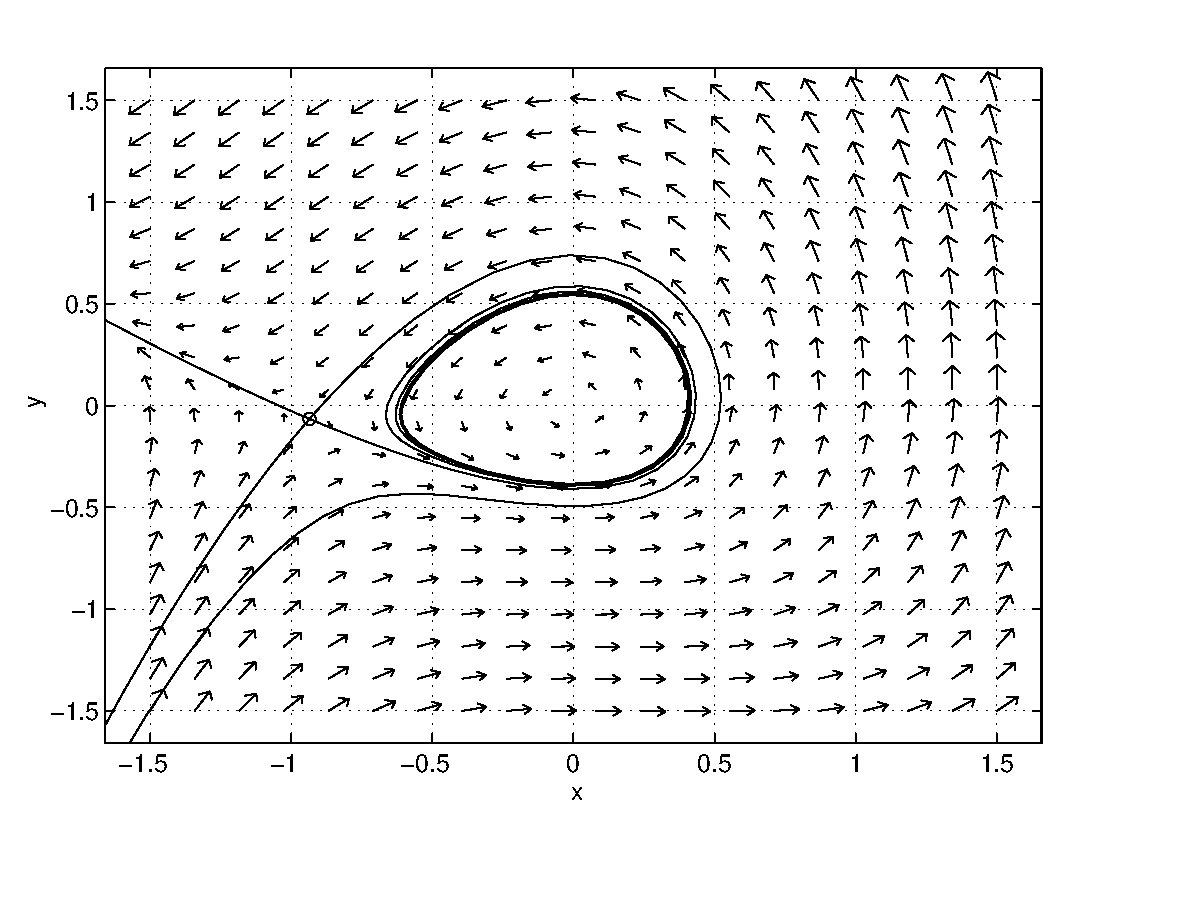
\psfig{file=../figures/homobif2.eps,height=2.0in}
           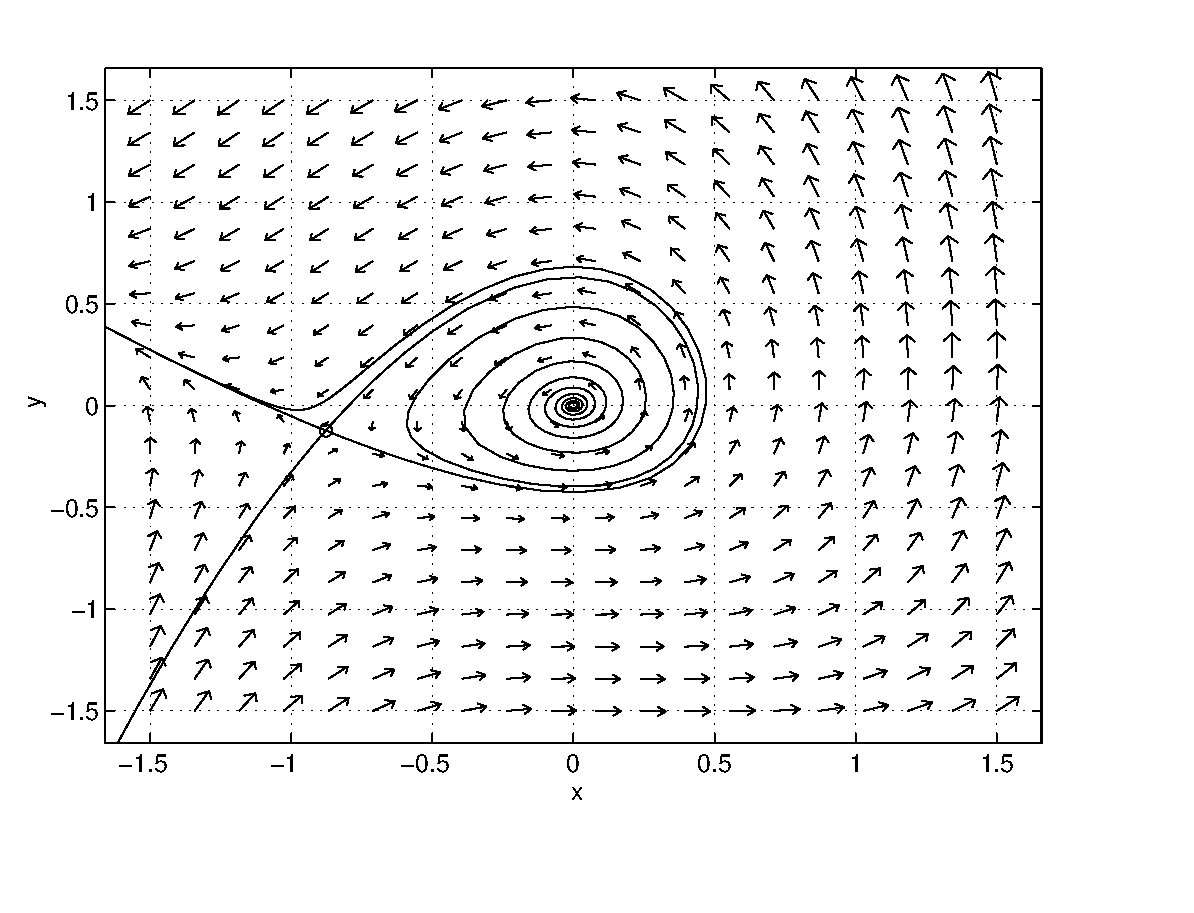
\psfig{file=../figures/homobif3.eps,height=2.0in}}
		\vspace*{-0.2in}		
	$\rho=-0.07$ \hspace{1.8in} $\rho=0.07$ 
		\hspace{1.8in} $\rho=0.14$
	  \caption{Phase planes for the differential equation 
	\protect\eqref{E:homobif}. }
           \label{F:homobif}
\end{figure*}

Use {\pplane} to plot the phase plane portraits of \eqref{E:homobif}
for $\rho=-0.07$, $\rho=0.07$, and $\rho=0.14$.  (These phase portraits 
are most easily drawn by having {\pplane} find the saddle point and
then plot the stable and unstable orbits.)  The phase portraits are 
displayed in Figure~\ref{F:homobif}.  

From the numerical calculations we see that a standard Hopf bifurcation 
to a stable limit cycle occurs as $\rho$ 
increases through $0$ --- but that limit cycle disappears by the
time $\rho=0.14$.   We discuss homoclinic bifurcations in more detail 
in Section~\ref{S:bifurcation}.  For the moment, just note that such 
transitions are possible.  In bifurcation diagrams, a homoclinic 
bifurcation  is indicated by having a branch of periodic solutions
terminate with a black dot.  In Figure~\ref{F:homobifdiag} we show the 
bifurcation diagram for the system of differential equations 
\eqref{E:homobif} for $\rho$ between $-0.1$ and $0.15$.  Note that there
are branches for two equilibria and a 
branch of limit cycles\index{branch of limit cycles} 
beginning at a Hopf bifurcation and ending at a homoclinic bifurcation.
In this particular bifurcation diagram we have labeled all pieces
of information including the equilibria and their types, the 
bifurcations and their types, and the limit cycles.


\begin{figure*}[htb]
           \centerline{%
           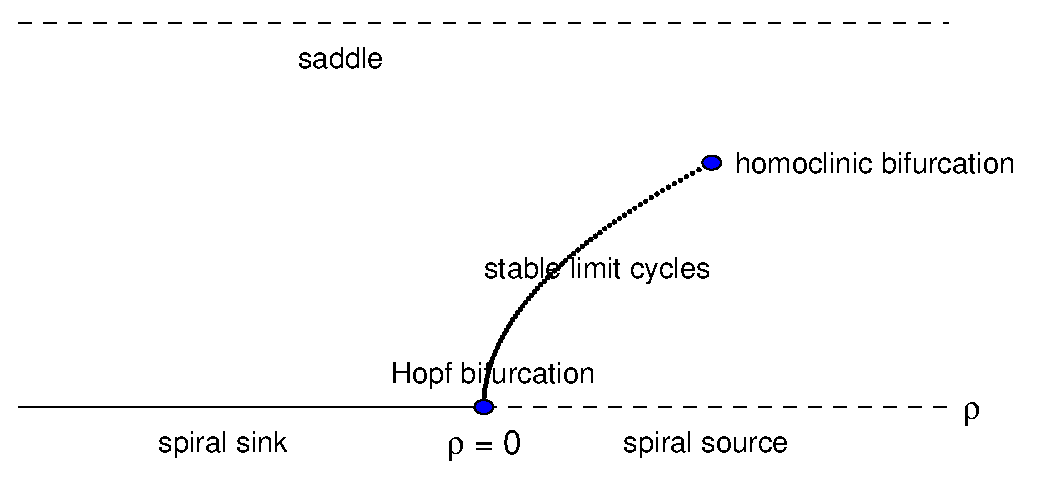
\psfig{file=../figures/homobifdiag.eps,height=2.5in}}
  \caption{Schematic bifurcation diagram for the differential equation
    \protect\eqref{E:homobif} indicating a branch of stable limit cycles
        ending in a homoclinic bifurcation.}
           \label{F:homobifdiag}
\end{figure*}
\index{diagram!bifurcation}

Homoclinic bifurcations are global bifurcations; the change in the phase 
portrait does not occur in a small neighborhood of an equilibrium.  For 
this reason we cannot detect homoclinic bifurcations analytically as we 
did for saddle-node bifurcations in \eqref{E:DCSN} and \eqref{E:DCSN2} and Hopf bifurcations in \eqref{E:NCHB}.




\subsection*{Reading Bifurcation Diagrams}

Planar systems of differential equations that model applications often
lead to complicated bifurcation diagrams.  We will see an example
of this complexity in Section~\ref{S:CSTR} when we study a model for a 
continuous flow stirred tank chemical reactor.  
Now we discuss the information contained in the hypothetical bifurcation 
pictured in Figure~\ref{F:hypo}. In words we describe the six bifurcations
contained in this hypothetical bifurcation diagram. 

\begin{figure}[htb]
           \centerline{%
           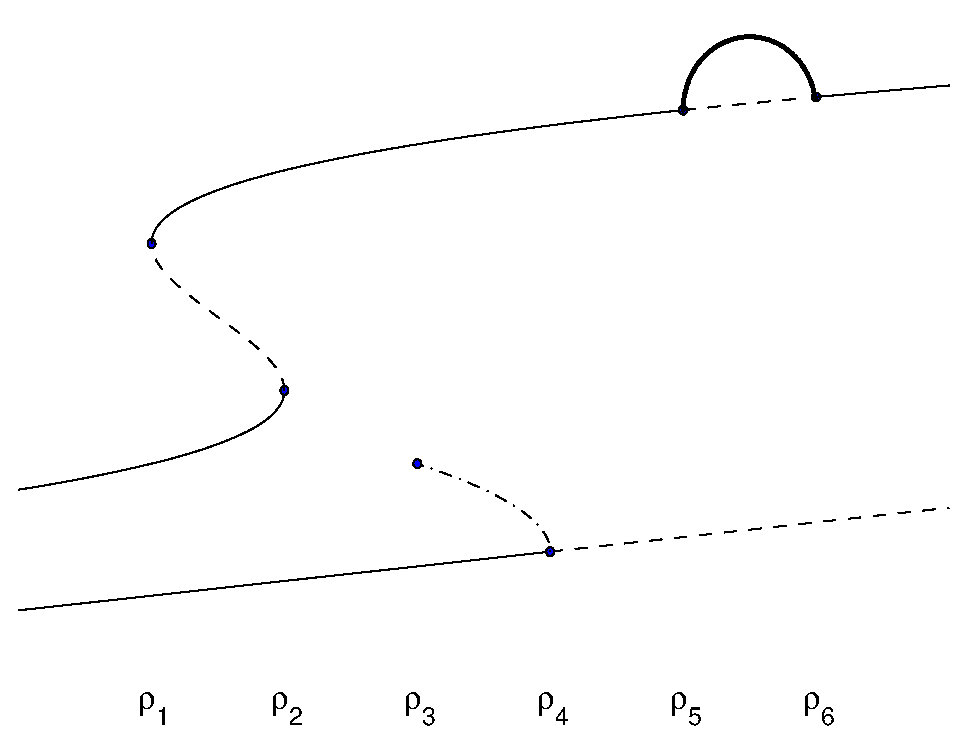
\psfig{file=../figures/hypo.eps,height=3.0in}}
  	   \caption{A hypothetical schematic bifurcation diagram for a planar 
	  system of differential equations with six bifurcation points.} 
           \label{F:hypo}
\end{figure}
\index{diagram!bifurcation}

For $\rho<\rho_1$
there are two stable equilibria.  There is a saddle-node bifurcation 
at $\rho_1$ where two additional equilibria --- one stable and one 
unstable --- are created.  At $\rho_2$ there is a second saddle-node 
bifurcation where two of the four equilibria disappear.  
\index{bifurcation!saddle-node}

As $\rho$ increases past $\rho_3$ a homoclinic 
bifurcation\index{bifurcation!homoclinic} produces an
unstable limit cycle that disappears at a 
Hopf bifurcation\index{bifurcation!Hopf} at $\rho_4$.  
Note that the equilibrium becomes unstable at $\rho_4$.
Hopf bifurcations also occur at $\rho_5$ and $\rho_6$.   A stable
limit cycle is created at $\rho_5$ and disappears at $\rho_6$.
\index{bifurcation!Hopf}

As you can see, a  bifurcation diagram is a shorthand method for recording
an exceptional amount of information.  In subsequent sections we develop 
some of theory needed to understand the changes that are to be expected 
at each bifurcation.  

\EXER

\includeexercises



\end{document}
